\newpage

\titleformat % design des titres des chapitres
{\chapter}
[display]
{\centering\normalfont\Large\scshape\bfseries}
{\rule[3pt]{0.15\linewidth}{3pt}\quad\chaptertitlename~\thechapter\quad \rule[3pt] {0.15\linewidth}{3pt}}
{0\baselineskip}%espace vertical entre chapitre et nom du chapitre
{\rule{\linewidth}{0.5pt}\break\Huge}
[\vspace{-0.5\baselineskip}\rule{\linewidth}{0.5pt}\vspace{0\baselineskip}]

\let\clearpage\relax% Stop LaTeX from going to a new page; and
\vspace*{5.5cm}%

\chapter{Etude generale du projet}
Le présent chapitre a pour but de définir les clés du travail
d’identification et planification du projet.

\newpage

\section{Périmètre du projet}
\subsection{Problématique générale}

Actuellement, il n’existe aucune solution pour la gestion d'effectif. Il est
pertinent de libérer le style classique adopté par les commerciaux et les responsables des
ressources humaines qui consiste à utiliser des documents « Excel » pour classifier tous les
acteurs matériaux ou humanitaires qui participent dans la construction d’un « Deal », et
faire des calculs manuels des coûts.
\\

Donc notre problématique majeure, nous devons définir d’une manière claire et précise les
besoins et les attentes d’un système d’information permettant d’automatiser les
remontées de l’équipe vers différentes entités, ainsi que la saisie des Deals, choix des
Squads, l’affectation des ressources et aussi la gestion de la relation client. D’une autre part garder la trace de tous les échanges afin de pouvoir établir des statistiques et prendre la décision du gain du deal.

\subsection{But du projet}

Le but de ce projet est de réaliser une solution power platform pour la facilitation et la gestion de la planification des effectifs. C’est un outil pour la digitalisation du processus de gestion des effectifs qui a pour vision de :

\begin{itemize}
  \item Un contrôle des coûts efficace nécessite une plate-forme robuste capable de rassembler des données à partir de différentes sources.
  \item Permettre aux account et service line de s'imbriquer conjointement sur les actions nécessaires à l'aide d'informations commerciales en temps quasi réel non disponibles dans les tableaux de bord de l'entreprise.
  \item Capacité à extraire les informations nécessaires pour répondre aux demandes des clients de manière agile et automatisée.
  \item Facilitez le niveau d'informations souhaité pour générer les bons résultats commerciaux.
\end{itemize}

Ma mission durant ce stage de fin d’études consiste à améliorer cela, les principaus module que j'ai developpé avec l'équipe BI sont:
\\
\begin{itemize}
  \item Accounth Growth form
  \item Accounth Run-Off form
  \item Accounth Migration
  \item Accounth Productivity
  \item Service Line Run-Off
  \item Service Line Migration Form
  \item Service Line Productivity Form
  \item DCT Form
  \item Rebalance Form
  \item Sub Contractor Conversion Form
  \item Sub Contractor Migration Form
  \item Sub Contractor Replacement Form
  \item Sub Contractor Productivity Form
\end{itemize}

\subsection{Livrables}
Le tableau suivant reprend les livrables du projet :

\begin{figure}[!h]
    \centering
    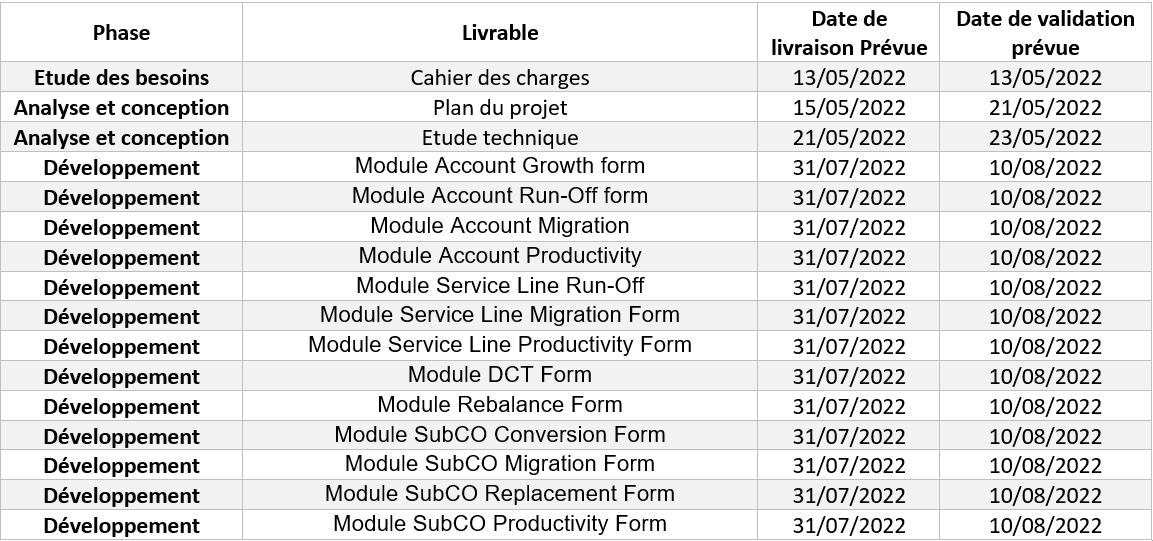
\includegraphics[scale=0.55,keepaspectratio]{Rapport de stage PFE chez DXC/figures/livrable.JPG}
    \caption{Les Livrables}
\end{figure}

\subsection{Registre de Gestion des Risques} 

Le “Registre de Gestion des Risques” sera créé et maintenu par le chef de projet
décrivant les risques de toutes natures pouvant affecter la bonne réalisation du projet et
détaillant leur probabilité de réalisation et la sévérité des impacts sur le projet. L’objectif de cette procédure de gestion des risques est d’en maîtriser autant que possible les effets et de permettre la définition et la mise en œuvre de mesures visant à en limiter les effets.

\newpage
\begin{figure}[!h]
    \centering
    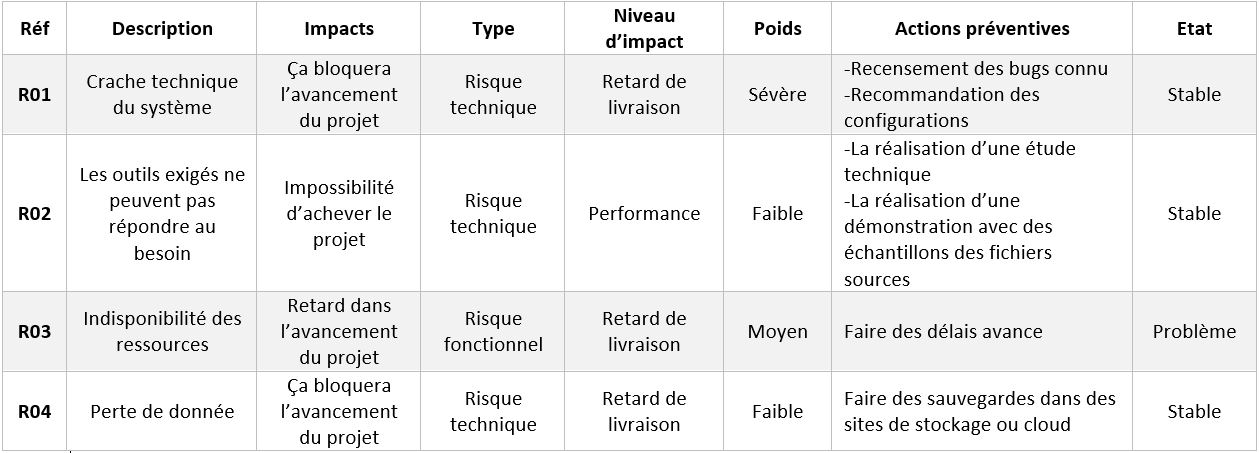
\includegraphics[scale=0.5,keepaspectratio]{Rapport de stage PFE chez DXC/figures/risques.jpg}
    \caption{Registre de Gestion des Risques}
\end{figure}

\subsection{Planification du projet}

Le projet était nouveau pour ma part, Il utilise power platform une technologie non abordée le long de mon parcours scolaire. Du coup, une planification rigoureuse s’est imposée pour prévoir le déroulement du projet. Grâce aux réunions tenues avec mon encadrant au sein de DXC, J'ai été éclairés sur les différentes étapes du projet ainsi que leurs séquencements.
\\\\
Le stage a débuté le 1er mars pour une durée de 6 mois. Il en résulte le planning
suivant :
\\
\begin{figure}[!h]
    \centering
    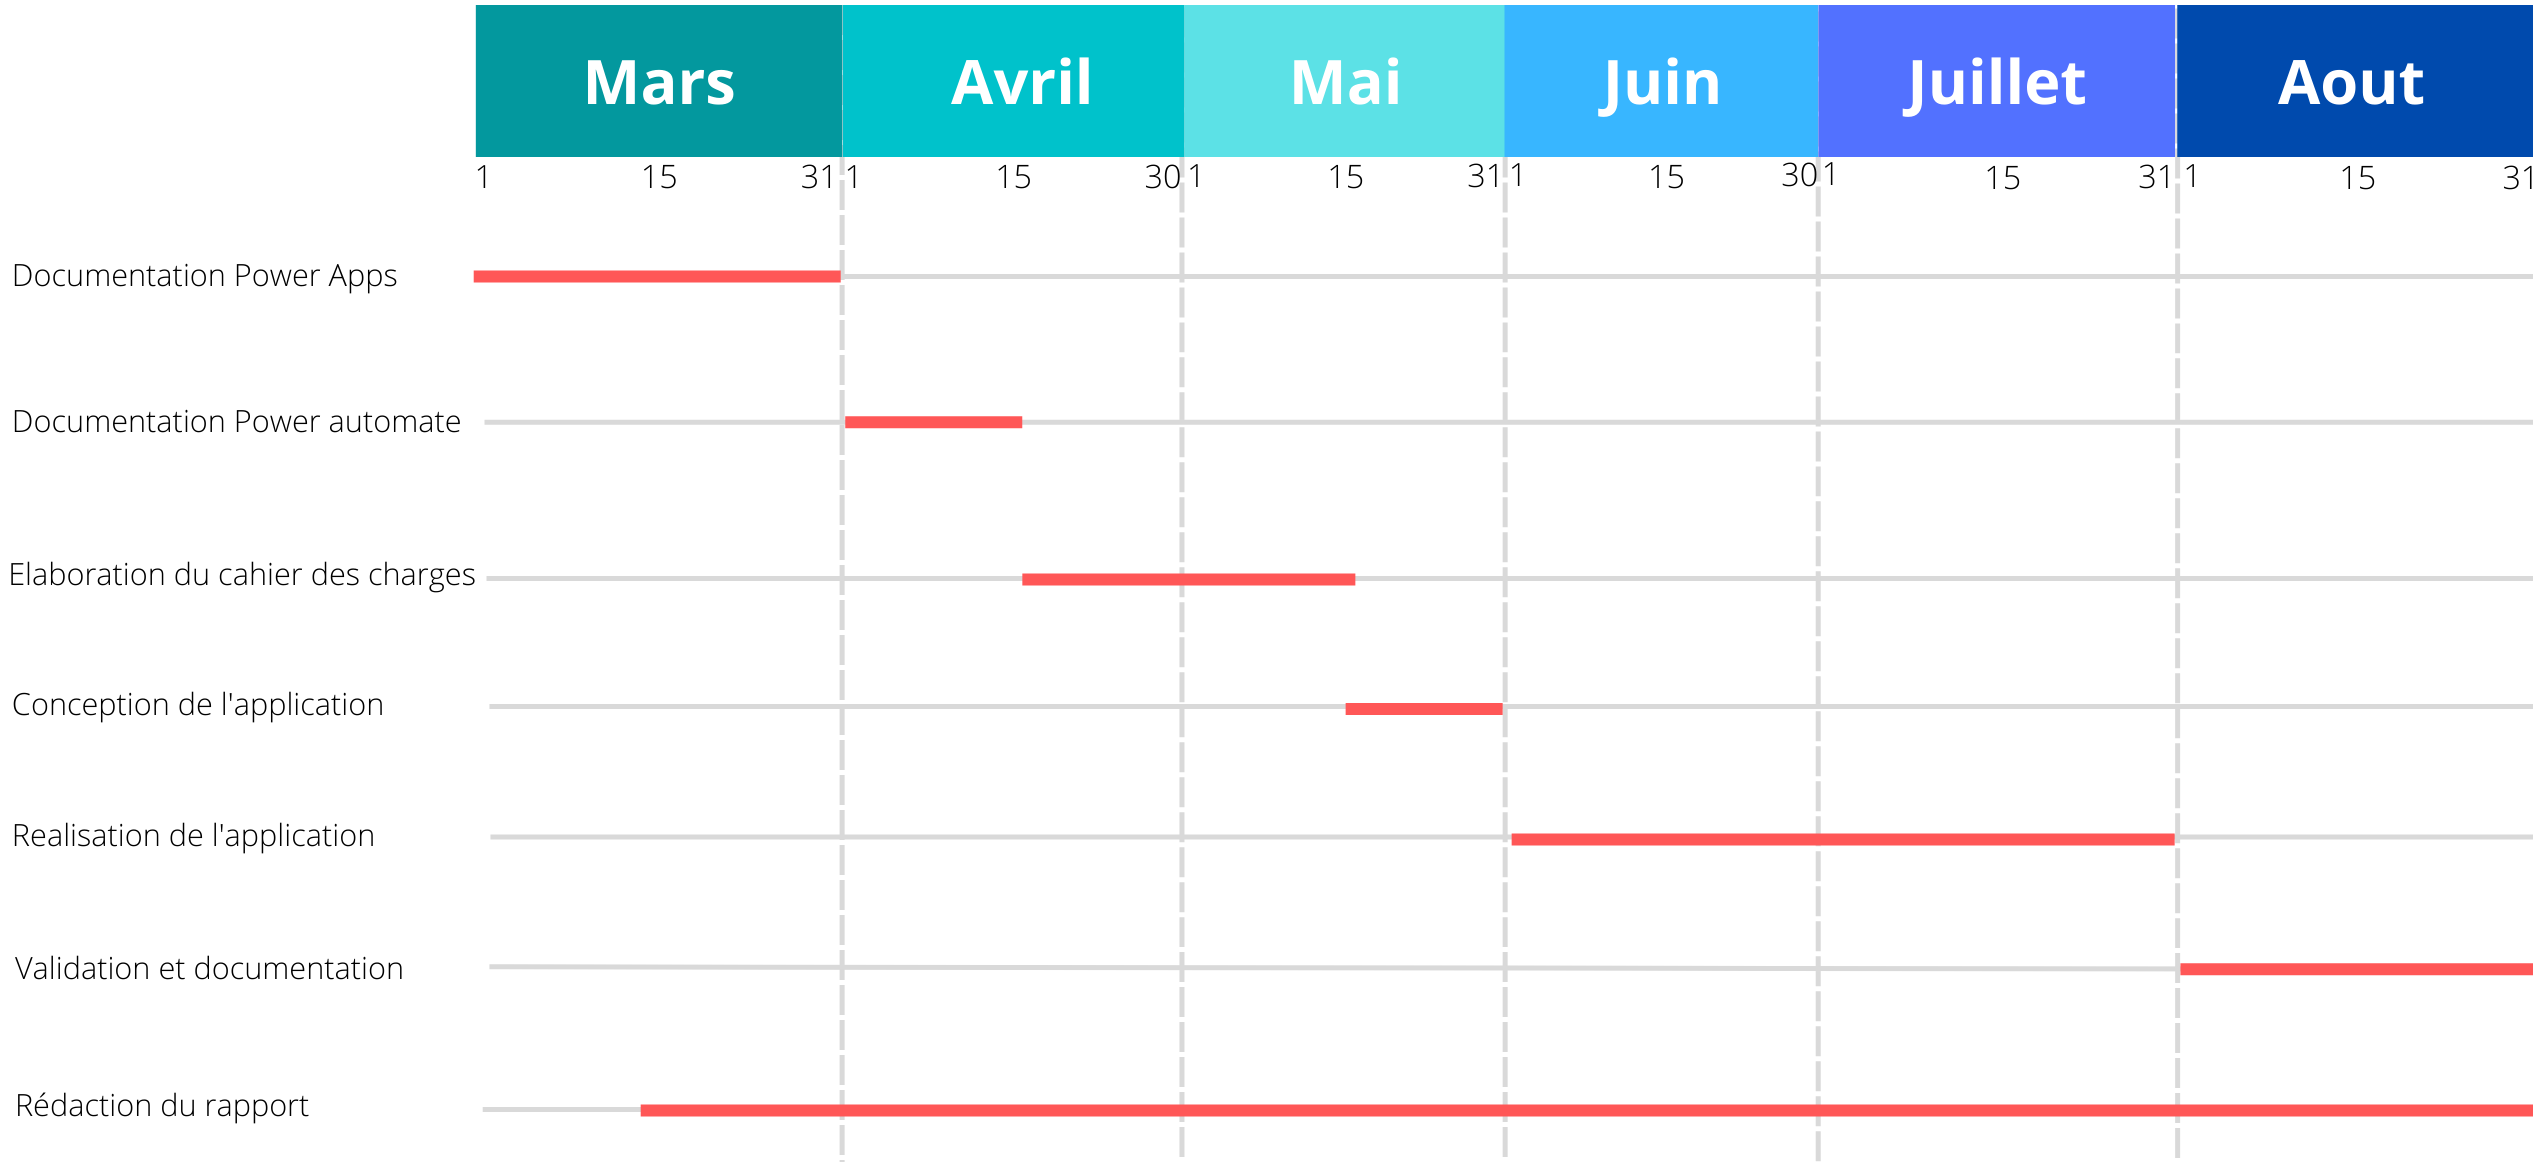
\includegraphics[scale=0.27,keepaspectratio]{Rapport de stage PFE chez DXC/figures/planification_projet_cropped.png}
    \caption{Diagramme de Gantt}
\end{figure}

\newpage
Le projet est partagé en trois grandes étapes : 
\\
\begin{itemize}
  \item La première est une phase de documentation dont les objectifs est de bien assimiler les différents composant de Microsoft Power Platform à savoir manipuler Power Apps et Power Automate.
  \item La phase de l'élaboration du cahier de charge, vu que le projet avait beaucoup de collaborateur cette dernière a pris du temps pour les mettre en accord sur les différentes fonctionnalités de l'application.
  \item La phase de conception de l'application
  \item La phase de réalisation de l'application où j'ai commencé par d'abord élaborer le frontend pour ensuite passer au backend en utilisant Power Apps et Power Automate.
  \item Finalement la validation de l'application par les différents membres de l'équipe ainsi que ça documentation.
\end{itemize}
\\
\section{Conclusion}

Dans ce chapitre j’ai présenté l’étude générale du projet ainsi que son but les differents livrable ainsi que la planification de ce dernier. Le chapitre suivant se concentrera sur l’étude des besoins du
projet.
